\paragraph{Objectives of the BATA subproject.}

\begin{figure}
\begin{center}
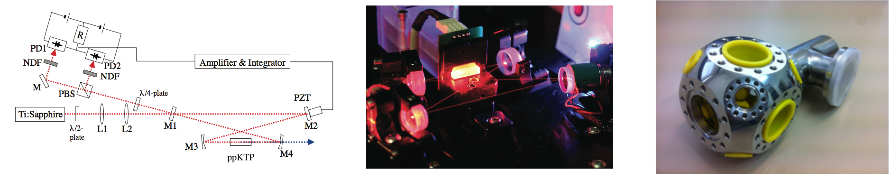
\includegraphics[width=0.99\textwidth]{img/blueLaser.png}
%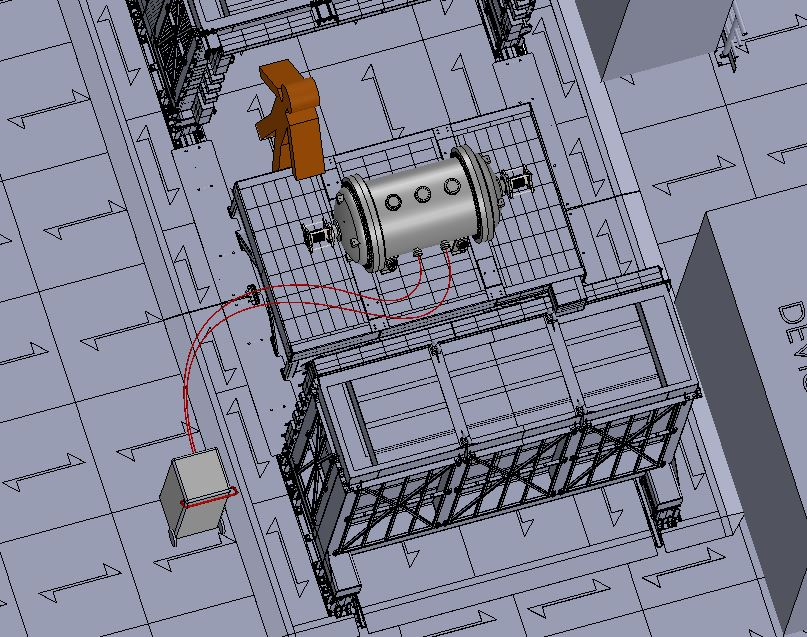
\includegraphics{img/CALIB_LSC_sources.jpg}
\caption{\small Left. Experimental set-up for resonant frequency doubling of a 
Ti:Sapphire laser using ppKTP. Right: the chamber for the prove-of-concept experiments, built at IFIC, and ready to be installed at CLPU.}
\label{fig:chamber}
\end{center}
\end{figure}

\begin{figure}[h!]
\begin{center}
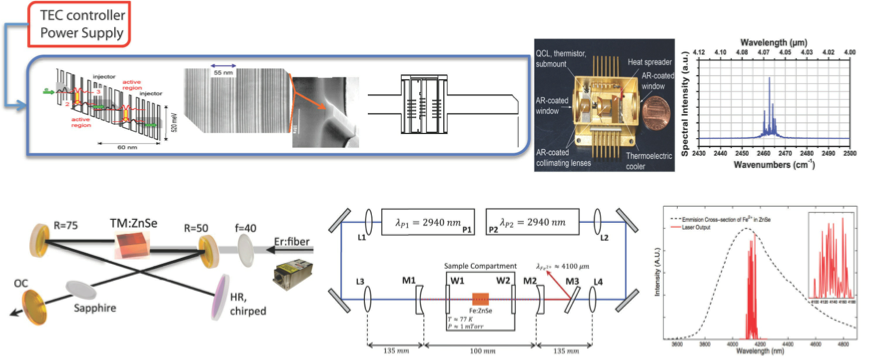
\includegraphics[width=0.99\textwidth]{img/MIR.png}
\end{center}
\caption{\label{Fig:MIR} (Top) Band theory of QCL, semiconductor material with physical bands and first device with laser spectrum at MIR. (Bottom) Schematic view of the TM:ZnSe laser design (two potential configurations with Er pumping laser) with potential tunable laser curve and free running emission. All MIR optics are made of CaF2, ZnSe and AR-coated at 2940 - 5000 nm) }
\end{figure}

The \BATA\ subproject will focus in the R\&D program needed to clearly establish the feasibility of tagging (e.g., detecting) the barium (Ba$^{++}$) ion produced in the double beta decay of xenon. 
%Demonstrating that an efficient detection of barium is possible in an \HPXE\ would imply that the NEXT technology could be upgraded to the ton scale while at the same time reducing the background by two or more orders of magnitude, resulting in a virtually background-free experiment with enormous possibilities of hitting a discovery. 

The \BATA\ program involves a set of proof-of-concept experiments. It also proposes the developments of a 4.1 $\mu$m laser, needed for the deshelving of the metastable state D. An attractive feature of such laser is its wide range of scientific and technological applications. CLPU is specially well suited to develop the technology.

The different objectives of this subproject are, therefore:

\begin{itemize}
	\item \textbf{Proof of principle experiment with Ba ions generated by means of an electrical discharge.}
	
	\item \textbf{Proof of principle experiment with Ba ions generated by an ion source.}	
	
%	\item \textbf{Proof of principle experiment with Ba ions generated by an ion source and with a magneto trap.}	
% In order to better control the experimental conditions, we will repeat the experiment but with the ions now confined in a magnetic trap. This trap will allow us to have an excellent degree of control over the experimental conditions and to approach the conditions that can be expected in the NEXT experiment. For instance we will carry out different measurements comparing the collected fluorescence signal as a function of the pressure of the Ba$^+$ ions and the pressure of the surrounding environment. These measurements are mandatory because the population dynamics is very sensitive to pressure, i.e., to collisions. 
%	
	\item \textbf{Proof of principle experiment with an additional laser for deshelving the D state.} A likely scenario is that the collisional induced decay between the metastable state D and the ground state S is either not effective or too slow for obtaining an appreciable fluorescence signal. In this situation the population is trapped in the metastable state D and the fluorescence cycle can not be closed. To avoid this difficulty, deshelving the D state may be needed.

\item \textbf{Development of a state-of-the-art 4.1\,$\mu$m laser}. Such a laser is needed for deshelving the D state, and laser emission in this mid-infrared region has many potential applications.

\end{itemize}

%\subsubsection*{\BATA\ subproject: Resources}
%
%For the successful development of this subproject, CLPU will provide the required human and technological resources. CLPU is the centre of reference in Spain regarding laser technology, and takes active part in several international and national projects. The leader of this subproject will be Alicia V. Carpentier who has a well recognised international trajectory in laser-matter interaction. Moreover, {\bf CLPU considers this project of high priority and consequently will offer the collaboration of all the scientific department} consisting of a multidisciplinar team with broad experience in laser technology and development, and laser-matter interaction. 
%
%Furthermore, CLPU will support this project with some of the already operating laser systems in its installation. This is extremely important because such systems usually cost of the order of several hundreds of thousand euros. The human resources needed to operate the laser systems will be provided by CLPU as well. For the construction of the ion source, and taking into consideration the specific requirements of this development, we will apply for an \emph{EXPLORA tecnología} in the 2014 call. 
%
%The budget of this subproject will be dedicated to: a) purchase small equipment for the proof-of-principle experiments; b) purchase a small commercial infrared laser for the initial deshelving experiment; c) develop a state-of-the-art, high power, very stable infrared laser to be used in a large system. It is important to insist that such a laser has many possible applications given the fact that its wavelength is not absorbed by the atmosphere as it lies in what is called the infrared atmospheric window.
%
%
%\subsubsection*{BATA subproject: schedule}
%
%
%
